
\documentclass[handout]{beamer}
\usepackage{pgfpages}
\usepackage[]{graphicx}
%\documentclass{beamer}
%\usepackage{beamerthemesplit}

\def\ce#1{\centerline{#1}}
\def\no{\noindent} 
\def\nl{\newline}
% -------
 \def\cblack{\color{black}}
 \def\cb{\color{blue}}
 \def\cred{\color{red}}
 \def\cy{\color{yellow}}
 \def\cg{\color{cyan}}
% -------
 \def\bs{\end{frame}\begin{slide}}
 \def\bi{\begin{itemize}[<+-| alert@+>]} 
 \def\ei{\end{itemize}}
 \def\i{\item} 
 
\def\t{\theta} 
\def\l{\lambda} 
\def\d{\delta} 

 \def\cblack{\color{black}}
 \def\cb{\color{white}}
 \def\cred{\color{yellow}}
 \def\cy{\color{yellow}}
 \def\cg{\color{green}}
% -------
\def\bs{\end{frame}\begin{slide}}
 \def\bi{\begin{itemize}[<+-| alert@+>]} 
 \def\ei{\end{itemize}}
 \def\i{\item} 


\def\t{\theta} 
\def\T{\Theta} 
\def\l{\lambda} 
\def\d{\delta} 
\def\e{\varepsilon} 
\def\s{\sigma} 
\def\ss{\sigma^2} 
\def\Sy{S_{yy}} 
\def\SS{\textsf{SS}} 
\def\N{\textsf{N}} 
\def\NG{\textsf{NG}} 
\def\Ga{\textsf{G}} 
\def\Sx{S_{xx}}
\def\Sxy{S_{xy}}
\def\ha{{\hat\alpha}}
\def\hb{{\hat\beta}}
\def\hy{{\hat y}}
\def\bx{\bar x}
\def\by{\bar y}

 \def\bi{\begin{itemize}} 
 \def\ei{\end{itemize}}
 \def\i{\item} 
 \def\tr{\textsf{tr}} 
\def\Wishart{\textsf{Wishart}}

\def\iid{\stackrel{iid}{\sim}}
\def\H{\textsf{H}} 
\def\E{\textsf{E}} 

\usepackage{bbold}
\def\I{\mathbb{1}}

\newcommand{\branchthree}[6]{
\left\{
	\begin{array}{ll}
		#1  & \mbox{if } #2 \\
		#3 & \mbox{if } #4 \\
		#5 & #6
	\end{array}
\right.
}

\title{STA 360/601: Bayesian and Modern Statistics}

\subtitle{Lecture 16: Bayesian hypothesis testing \& Bayes factors}

\author{Jeff Miller}

\institute{Department of Statistical Science, Duke University}

\date{Friday, October 17, 2014}

\graphicspath{{figures/}}

\begin{document}

\frame{\titlepage}

%\section[Outline]{}
%\frame{\tableofcontents}



\begin{frame}
\frametitle{Bayesian hypothesis testing}
\begin{itemize}
\item Problem: You have two or more competing hypotheses $\H_0,\H_1,\dotsc$, and want to consider the evidence in favor of each, based on some data.
\item Examples:
\begin{enumerate}
\item Does drug X reduce the risk of stroke ($\H_1$) or not ($\H_0$)?
\item Does Patient X have disease Y ($\H_1$) or not ($\H_0$)?
\item Does the Higgs boson exist ($\H_1$) or not ($\H_0$)?
\item You are Gregor Mendel. Which of several models of trait inheritance $\H_0,\H_1,\dotsc,\H_m$ is correct?
\item Data on 5000 subjects was collected over 60 years. Which variables are predictive of heart disease risk? (Each subset of variables is a competing hypothesis.)
\end{enumerate}
\end{itemize}
\end{frame}


\begin{frame}
\frametitle{A simple example}
\begin{itemize}
\item Data: $X_1,\dotsc, X_n\iid \N(\mu,\sigma^2)$, where $\sigma$ is known.
\item Hypotheses: $\H_0:\mu = 0$ versus $\H_1:\mu\neq 0$
\item Same setup as a classical frequentist hypothesis test.
\item Let's say the data is
$$x = (x_1,\dotsc,x_8) = (0.8, -0.4, 0.1, 0.0, 1.2, 0.8, 1.0, 0.9).$$
 What is your intuitive judgment of the plausibility of $\H_0$ and $\H_1$?
\item What would be a natural Bayesian approach? Any ideas?
\end{itemize}
\end{frame}


\begin{frame}
\frametitle{A Bayesian approach}
\begin{itemize}
\item Put a prior on the hypotheses, say, $p(\H_0)=\pi$ and $p(\H_1)=1-\pi$.
\item Under $\H_0:\mu = 0$, the data is simply $\N(0,\sigma^2)$.
\item Under $\H_1:\mu\neq 0$, we don't know $\mu$, so let's put a prior on it: $\mu\sim\N(0,\sigma_1^2)$.
(Technically, perhaps we should exclude the point $\mu=0$ from the prior, but it makes no difference since this has probability zero anyways.)
\item Now, we want to know the posterior probabilities $p(\H_0|x)$ and $p(\H_1|x)$ where $x =(x_1,\dotsc,x_n)$.
% \item Since $\H_0$ and $\H_1$ are mutually exclusive, $p(\H_0|x) + p(\H_1|x) = 1$, so we only need to compute one of $p(\H_0|x)$ and $p(\H_1|x)$.
\item By Bayes' rule, $p(\H_k|x)\propto p(x|\H_k)p(\H_k)$. So, we need $p(x|\H_0)$ and $p(x|\H_1)$ (the \emph{marginal likelihoods}).
\end{itemize}
\end{frame}


\begin{frame}
\frametitle{Computing the marginal likelihoods}
\begin{itemize}
\item $\H_0$ is easy: $p(x|\H_0) =\prod_{i = 1}^n \N(x_i\mid 0,\sigma^2)$
\item \dots and $\H_1$ is not too hard:
\begin{align*}
p(x|\H_1) &= \int p(x|\mu,\H_1) p(\mu|\H_1) d\mu\\
& =\int \Big(\prod_{i = 1}^n \N(x_i\mid \mu,\sigma^2)\Big) \N(\mu\mid 0,\sigma_1^2) d\mu\\
& = \mbox{(typical Gaussian integral\dots complete the square, etc.)} \\
& = \frac{s}{\sigma_1}\exp\big(\tfrac{1}{2}m^2/s^2\big) \prod_{i = 1}^n \N(x_i\mid 0,\sigma^2),
\end{align*}
where $1/s^2 = n/\sigma^2+1/\sigma_1^2$ and $m =(s^2/\sigma^2)\sum_i x_i$.
\end{itemize}
\end{frame}


\begin{frame}
\frametitle{Outcome for our simple example}
\begin{itemize}
\item Our data is
$$x = (x_1,\dotsc,x_8) = (0.8, -0.4, 0.1, 0.0, 1.2, 0.8, 1.0, 0.9).$$
\item Let's suppose $p(\H_0) = p(\H_1) = 1/2$, $\sigma = 1$, and $\sigma_1 = 1$.
\item Plugging the marginal likelihood and prior into $p(\H_k|x)\propto p(x|\H_k)p(\H_k)$ we get
$$ p(\H_0|x) = 0.506 \mbox{ and } p(\H_1|x) = 0.494.$$
\item So, basically, we have no idea.
\end{itemize}
\end{frame}


\begin{frame}
\frametitle{Decisions, decisions, \dots}
\begin{itemize}
\item Suppose we have to choose one of the hypotheses.
\item Suppose that when we choose $d$ and the truth is $h$, we incur a loss $L(h,d)$.
\item Since we have put a prior on $h$, we may as well consider it as a random variable, $H$.
\item The \emph{posterior expected loss} associated with choosing $d$ given data $x$ is
$$\E\big(L(H,d)\mid x\big) = \sum_h L(h,d) p(H=h\mid x) $$
where the sum is over all hypotheses $h =\H_0,\H_1,\dotsc$.
\end{itemize}
\end{frame}


\begin{frame}
\frametitle{Example: 0 - 1 loss}
\begin{itemize}
\item \emph{0 - 1 loss} is the loss function $L(h,d) =\I(h \neq d)$, i.e., you lose 1 if wrong, 0 if right.
\item The posterior expected loss in this case is
\begin{align*}
\E\big(L(H,d)\mid x\big) &= \sum_h L(h,d) p(H=h\mid x) \\
&= \sum_h \I(h \neq d) p(H=h\mid x) \\
&= 1 - p(H=d\mid x).
\end{align*}
\item So, to minimize our posterior expected loss, the optimal decision $d^*$ (under 0 - 1 loss) is the hypothesis with highest posterior probability $p(H = d|x)$.
\item In the case of two hypotheses, $\H_0$ and $\H_1$,
$$ d^* = \branchthree{\H_0}{p(\H_0|x)>1/2}{\H_1}{p(\H_1|x)>1/2}{\mbox{either}}{\mbox{otherwise.}} $$
\end{itemize}
\end{frame}


\begin{frame}
\frametitle{A few remarks}
\begin{itemize}
\item If $L(h,d)$ is not 0 - 1 loss, the optimal decision will not necessarily be the hypothesis with highest posterior probability.
\item The Bayesian hypothesis testing approach described above is very different than frequentist hypothesis testing.
\item For frequentist hypothesis testing of $\H_0$ versus $\H_1$:
\begin{itemize}
\item The usual approach is to minimize Type II errors (choosing $\H_0$ when $\H_1$ is true) subject to an upper bound on the probability of Type I error (choosing $\H_1$ when $\H_0$ is true).
\item There is an asymmetry in the frequentist approach: $\H_0$ is a \emph{null hypothesis}, i.e., a default position (the reigning champion), and $\H_1$ is an \emph{alternative hypothesis} (the challenger).
\item Metaphor: It is like a criminal trial, in which the defendant is presumed innocent ($\H_0$) unless proven guilty beyond all reasonable doubt ($\H_1$).
\end{itemize}
\item The Bayesian approach does not have this asymmetry, allowing for a more balanced approach to minimize overall loss.  However, as always, the outcome depends on the prior.
\end{itemize}
\end{frame}



\begin{frame}
\frametitle{Bayes factors}
\begin{itemize}
\item Bayes factors provide a way to be a little less dependent on the prior.
\item The \emph{Bayes factor} in favor of $\H_1$ over $\H_0$, for data $x =(x_1,\dotsc,x_n)$, is
$$ B_{10} = \frac{p(x|\H_1)}{p(x|\H_0)}. $$
\item Note that this doesn't depend on $p(\H_0)$ or $p(\H_1)$ \dots
\item \dots but it does still depend on the priors we choose for parameters required to define the distribution of $x$ given $\H_0$ or $\H_1$ (e.g., $\mu$ in our simple example).
% \item Obviously, $B_{01} = 1/B_{10}$.
\item When $B_{10}>1$, this is evidence in favor of $\H_1$, when $B_{10}<1$, it is evidence in favor of $\H_0$.
\item Some have suggested scales for interpreting Bayes factors, e.g., 10 -- 30 is ``strong evidence'', but this is purely heuristic and not universally accepted.
\end{itemize}
\end{frame}


\begin{frame}
\frametitle{Some properties of Bayes factors}
\begin{itemize}
\item In the case of two competing hypotheses, the Bayes factor is related to the posterior probability as follows:
\begin{align*}
p(\H_0|x) & =\frac{p(x|\H_0) p(\H_0)}{p(x|\H_0) p(\H_0) + p(x|\H_1) p(\H_1)}\\
& =\frac{1}{1+\frac{p(x|\H_1)p(\H_1)}{p(x|\H_0) p(\H_0)}}\\
& =\frac{1}{1+\mbox{Bayes factor $\times$ Prior odds}}
\end{align*}
\item Also, ``Posterior odds = Bayes factor $\times$ Prior odds'', i.e.,
$$\frac{p(\H_1|x)}{p(\H_0|x)} = B_{10} \frac{p(\H_1)}{p(\H_0)}. $$
\end{itemize}
\end{frame}


\begin{frame}
\frametitle{Back to our example}
\begin{itemize}
\item Data: $x = (0.8, -0.4, 0.1, 0.0, 1.2, 0.8, 1.0, 0.9).$
\item $p(\H_0) = p(\H_1) = 1/2$, $\sigma = 1$, and $\sigma_1 = 1$.
\item Posterior probabilities:
$$ p(\H_0|x) = 0.506 \mbox{ and } p(\H_1|x) = 0.494.$$
\item Bayes factors:
$$ B_{10} = \frac{p(x|\H_1)}{p(x|\H_0)} = 0.98$$
$$ B_{01} = \frac{p(x|\H_0)}{p(x|\H_1)} = 1.02$$
\end{itemize}
\end{frame}



\begin{frame}
\frametitle{Sensitivity to the prior}
\begin{itemize}
\item Bayes factors can depend strongly on the prior on parameters (e.g., $\mu$ in our example).
\item In our example, the prior standard deviation $\sigma_1$ of $\mu$ given $\H_1$ has a significant effect on the Bayes factor:
\centerline{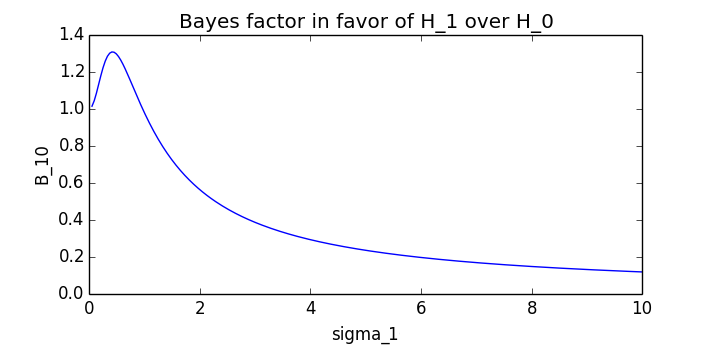
\includegraphics[width=0.8\textwidth]{Bayes_factors.png}}
\item In particular, $B_{10}\to 0$ as $\sigma_1\to\infty$.
\item Improper priors CANNOT be used here.
\end{itemize}
\end{frame}


\begin{frame}
\frametitle{Lindley's ``paradox''}
\begin{itemize}
\item This sensitivity is the issue underlying Lindley's ``paradox'' (which is, as usual, not actually a paradox).
\item The original ``paradox'' is that it is possible for very reasonable frequentist and Bayesian approaches to give contradictory answers about which hypothesis is favored by the evidence.
\item e.g., frequentist rejects $\H_0$ while Bayesian finds strong evidence for $\H_0$.
\item This underlying issue also shows up in Bayesian models over variable-dimension parameter spaces, e.g., mixture models.
\end{itemize}
\end{frame}


\begin{frame}
\frametitle{Non-monotonicity wrt sample size}
\begin{itemize}
\item Another thing to be careful of is that Bayes factors can be non-monotone in the sample size $n$.
\item Example: Same as before, but with $\sigma_1 = 5$ and $X_1,\dotsc,X_n\iid \N(0.1,1)$. Plot is averaged over many samples:
\centerline{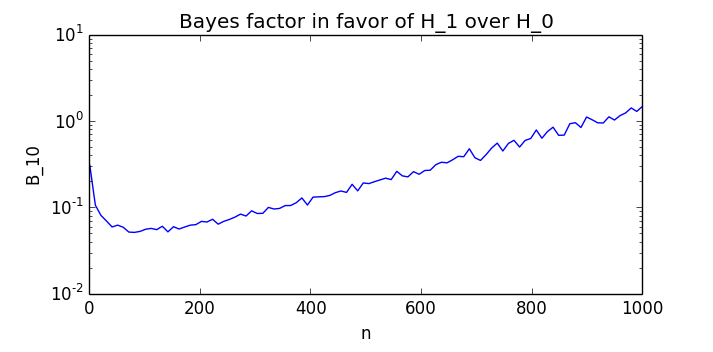
\includegraphics[width=0.8\textwidth]{non-monotone.png}}
\item $\H_1$ is true, but if we only had 100 samples, we would only see $B_{10}$ decreasing down to $\approx 0.05$, seeming to suggest that it is converging to $0$, and we might mistakenly be convinced of $\H_0$.
\end{itemize}
\end{frame}


\begin{frame}
\frametitle{Remarks}
\begin{itemize}
\item The Bayesian approach allows for principled (but subjective) decision-theoretic hypothesis testing.
\item Also, the Bayesian approach extends naturally to more complicated models.
\item The prior really matters here --- only trust the results to the extent that you trust the prior.
\item It's a good idea to do a sensitivity analysis: vary the prior and see how the result changes.
\item Careful: Bayes factors can be non-monotone in $n$.
\end{itemize}
\end{frame}


\begin{frame}
\frametitle{Homework exercise}
\begin{itemize}
\item You have data from an experiment collecting cell counts for a control group and treatment group.
\item Control group:
$$ x_{1:n} = (204,  215, 182,  225,  207,   188,  205,  227,  190,  211, 196,  203) $$
\item Treatment group:
$$ y_{1:m} = (211, 233, 244,  241,  195,  252,  238,  249,  220,  213)$$
\item The counts are assumed to be Poisson distributed.  
\item There are two hypotheses, $\H_0$: Poisson with same mean, vs. $\H_1$: Poisson with different means.
\end{itemize}
\end{frame}


\begin{frame}
\frametitle{Homework exercise (continued)}
\begin{itemize}
\item Model this as follows.
\item $p(\H_0) = 3/4$, $p(\H_1) = 1/4$. 
\item Under $\H_0$: $X_1,\dotsc,X_n,Y_1,\dotsc,Y_m\sim \mathsf{Poisson}(\lambda)$ i.i.d.\ given $\lambda$, and $\lambda\sim\mathsf{Gamma}(a,b)$ where $a=4=$ shape and $b=0.02=$ rate (i.e., $\lambda$ has pdf $b^a\lambda^{a-1}\exp(-b\lambda)/\Gamma(a)$).
\item Under $\H_1$: $X_1,\dotsc,X_n\sim \mathsf{Poisson}(\lambda_c)$ i.i.d.\ given $\lambda_c$, and $Y_1,\dotsc,Y_m\sim \mathsf{Poisson}(\lambda_t)$ i.i.d.\ given $\lambda_t$, and $\lambda_c,\lambda_t\sim\mathsf{Gamma}(a,b)$ independently, with the same $a,b$ as above.
\item Compute $p(\H_k|x,y)$ for $k = 0,1$. Compute $B_{10}$. 
\item Compute the prior odds and posterior odds. Interpret your results.
\item Does the prior on the $\lambda$'s appear to be reasonable (judging by the data)?  Why or why not?  Try different values of $a$ and $b$ and interpret what you see.
\end{itemize}
\end{frame}







\begin{frame}
\frametitle{Further reading}
\begin{itemize}
\item Kass \& Raftery, \emph{Bayes factors}, JASA, 1995.
\end{itemize}
\end{frame}






 
\end{document}








